%1234567890123456789012345678901234567890123456789012345678901234567890123456789
%         1         2         3         4         5         6         7        8

\documentclass[runningheads,a4paper]{llncs}
\usepackage{amssymb}
\setcounter{tocdepth}{3}
\usepackage{graphicx}
\usepackage{amssymb}
\usepackage[utf8]{inputenc}
\usepackage{url}

% \usepackage{breakurl}
\usepackage{float}
\usepackage{amsmath}
\usepackage{graphicx}
\usepackage[tight]{subfigure}
\usepackage{wrapfig}

\usepackage{lipsum}

\newcommand{\robospecs}{%
  \newpage%
  \pagenumbering{gobble}%
% \pagestyle{fancy}%
% \fancyhf{}%
%  \chead{$|$}
% \rhead{\footnotesize\thetitle}%
% \lhead{\footnotesize\theauthor}%
% \rfoot{Robot software and hardware specification sheet}%
}


\newcommand{\teamori}{Team ORIon}
\newcommand{\competitionyear}{2022}
\newcommand{\competitioncountry}{Thailand}
\newcommand{\robocuptitleshort}{RoboCup \competitionyear}

\usepackage{hyperref}
\hypersetup{
    colorlinks=true,
    linkcolor=black,
    anchorcolor=black,
    urlcolor=black,
    citecolor=black,
    filecolor=black
}
%https://www.youtube.com/watch?v=sZ_oqFDUsnM
\begin{document}

\authorrunning{Ricardo Cannizzaro et al.}

\title{\teamori\ --- 2022 Team Description Paper}

\author{Ricardo Cannizzaro \and Clarissa Costen \and Matthew Budd \and Shu Ishida \and Marc Rigter \and Ioannis Havoutis \and Nick Hawes \and Lars Kunze \and Bruno Lacerda}
\institute{Oxford Robotics Institute, Dept. of Engineering Science, University of Oxford, UK \\
\texttt{orion@oxfordrobotics.institute} \\
\url{https://ori.ox.ac.uk/student-teams/team-orion}}

\maketitle

%%%%%%%%%%%%%%%%%%%%%%%%%%%%%%%%%%%%%%%%%%%%%%%%%%%%%%%%%%%%%%%%%%%%%%%%%%%%%%%%%%%%

\begin{abstract}
This document outlines the approach \textit{\teamori} will take to the RoboCup@Home 2022 (DSPL).
Our first experience competing with Toyota's Human Support Robot (HSR) was at the World Robot Summit (WRS) 2018, where we competed in the Partner Robot Challenge. We have since competed at RoboCup 2019 in the DSPL @Home league. Due to the coronavirus pandemic, we were unfortunately unable to compete in the 2020 and 2021 competitions. However, \textit{\teamori} will return to the competition in 2022 with a refreshed and revamped team.
Our research interests are centred around long-term autonomy; mobility and whole body motion planning; causal reasoning and knowledge representation; and trustworthy and explainable AI.
Advances in these directions will enable service robots to interact with humans and complete useful everyday tasks in typical household settings, as well as other applications including autonomous inspection tasks and autonomous road vehicles. 
We aim to demonstrate robust and intelligent autonomous behaviour, that uses experience to learn and refine a growing set of robot skills, on the HSR.
\end{abstract}


%%%%%%%%%%%%%%%%%%%%%%%%%%%%%%%%%%%%%%%%%%%%%%%%%%%%%%%%%%%%%%%%%%%%%%%%%%%%%%%%%%%%

%The TDP is an 8-pages (+ annex) long scientific paper, detailing information on the technical and scientific approach of the team's research, while including also the following:
%\begin{itemize}
%	\item \checkmark Innovative technology and scientific contribution
%    \item \checkmark Focus of research/research interests
%    \item \checkmark Re-usability of the system for other research groups
%    \item \checkmark Applicability of the robot in the real world
%	\item \checkmark DSPL and SSPL: When the robot depicted in the TDP or Team Video is different from the league's standard one, the TDP must clearly state how the addressed approach and described software will be adapted to the standard platform robot.
%\end{itemize}

%Here are some references that can be relevant to our story:
%\cite{havoutis13ijrr,Winkler2015,havoutis15clawar,Mastalli2015,Havoutis16SSRR,Zeestraten2017-RAL,Havoutis17ICRA,Zeestraten17IROS,Mastalli17ICRA}.

\section{Introduction}

\textit{\teamori{}} is a student robotics competition team created in 2018 within the Oxford Robotics Institute (ORI) at the University of Oxford. 
The team consists of undergraduate and graduate students, and is supported by robotics postdoc researchers, principal investigators, and other faculty members of the ORI. 
We come from a strong research institute with seminal work in mobile autonomy and machine learning. The ORI has a significant track record in \emph{field robotics} and real-world trials of autonomous systems.
Further, the ORI also has a team of professional hardware and software engineers. This experience and support is leveraged to create a robotics competition team with a solid foundation to deliver a strong performance in the RoboCup competition.

\subsection{Past Competition Involvements}
The RoboCup@Home league provides a challenging environment and complex tasks to which new and existing ORI research can be applied. 
Since acquiring our Toyota Human Support Robot (HSR) in 2018, we have competed in the Partner Robot Challenge of WRS; we also competed in the 2019 RoboCup@Home competition, placing $6^{th}$ out of 10 on our first attempt at the competition (see Figure~\ref{fig:pastcompetitions}). 
The HSR robot allows us to focus on developing the
intelligence required for successfully completing complex tasks, 
without the added burden of building and maintaining a custom platform. 
Competing in the \robocuptitleshort\ event will allow us to demonstrate the capabilities presented in this document and will provide valuable experience for our future participations.

\subsection{Public Outreach}
Our team also run robot demonstrations to the public at outreach events, such as the Goodwood Festival of Speed, University open days, and the Oxford Science and Ideas Festival, to promote greater awareness and interest in STEM, robotics, and AI to the wider public. In October 2019, we demonstrated the HSR for His Royal Highness Prince William at the ORI to celebrate the opening of a new college building \cite{PrinceWilliamArticle} (see Figure~\ref{fig:outreach}).

\begin{figure}[tb]
	\begin{center}
  		\includegraphics[width=.41\columnwidth, clip, trim=0 0ex 0ex 50ex]{images/hsr_grasping.jpg}
  		\includegraphics[width=.49\columnwidth, clip, trim=0 0ex 0ex 50ex]{images/robocup_team.jpg}
	\end{center} 
	\caption{\emph{Left:} Team ORIon's HSR grasping a plant at the World Robot Summit (WRS) 2018 in Tokyo, Japan. \emph{Right:} Team ORIon at RoboCup@Home (WRS) 2019 in Sydney, Australia.}
	\label{fig:pastcompetitions}
\end{figure}

\begin{figure}[tb]
	\begin{center}
		\includegraphics[width=.20\columnwidth, clip, trim=0 0ex 0ex 0ex]{images/goodwood_hsr_coffee.jpg}
		\includegraphics[width=.39\columnwidth, clip, trim=20ex 0ex 0ex 0ex]{images/goodwood_demo_with_child.jpg}
		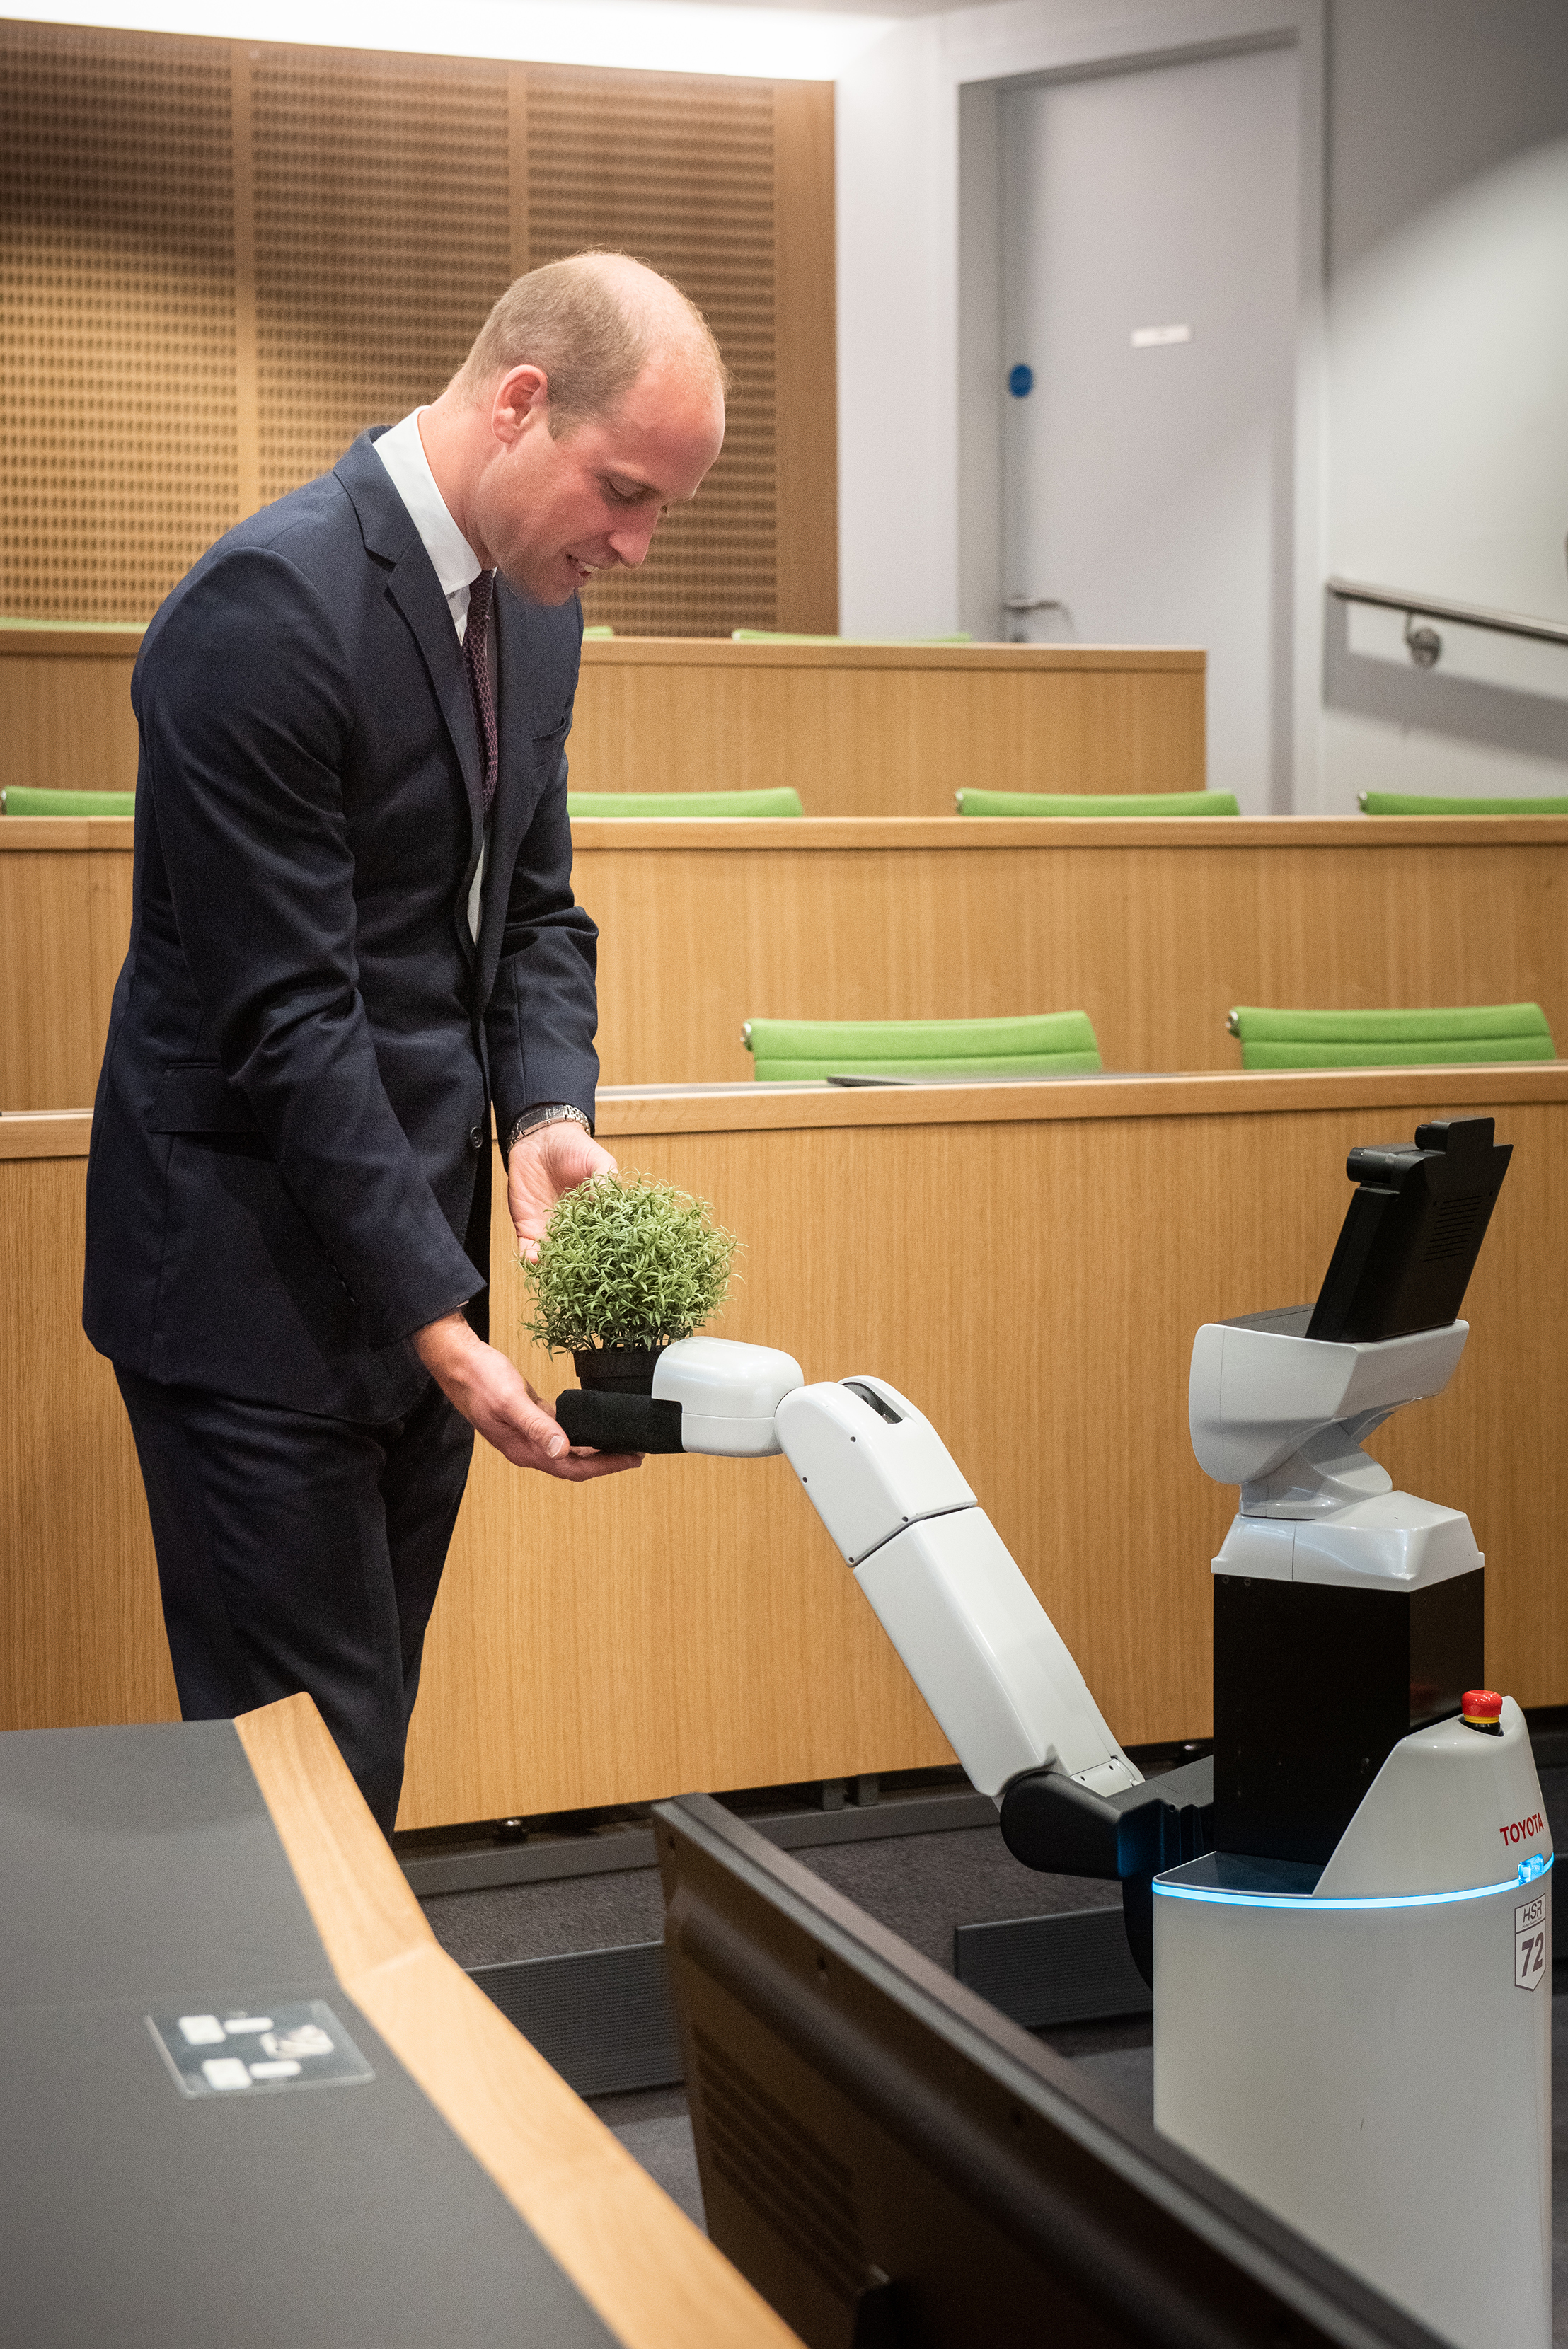
\includegraphics[width=.214\columnwidth, clip, trim=0ex 0ex 0ex 15ex]{images/keble_college_duke_of_cambridge_hb_allen_centre.jpg}
	\end{center} 
	\caption{\emph{Left, Middle:} Team ORIon demonstrating the HSR to the public at the 2021 Goodwood Festival of Speed. \emph{Right:} Demonstrating the HSR for HRH Prince William.}
	\label{fig:outreach}
\end{figure}


\section{Team Composition}
The team is led by ORI PhD student Ricardo Cannizzaro, and is composed into five sub-teams to manage different robot sub-systems: task-level planning, perception, manipulation, human-robot interaction, and semantic mapping. The core team for 2022 will be Oxford University PhD student sub-team leaders (Clarissa Costen, Matthew Budd, Shu Ishida, Marc Rigter), as well as PhD and undergraduate team members. The sub-team responsibilities and team members are described further on the \teamori website\footnote{\url{https://ori.ox.ac.uk/student-teams/team-orion/meet-the-team}}.
Since the start of the academic calendar in September (and following a substantial period of reduced activity due to the coronavirus pandemic), the team has made a large effort to recruit and train new team members, and review and consolidate existing robot functionality to prepare for the \robocuptitleshort\ competition. 

The team is supported by ORI principal investigators Dr. Lars Kunze, who has a strong research focus on scene understanding and semantic mapping, causal reasoning, and explainable and trustworthy AI; Prof. Nick Hawes, who has extensive background in intelligent autonomous robots that can work with or for humans in uncertain environments; and Dr. Ioannis Havoutis, an expert in combining motion planning with machine learning.

\section{Research, Capabilities and Goals}

% TODO - replace with more relevant figure showing original research or novel functionality
\begin{figure}[tb]
  \begin{center}
    \includegraphics[width=.43\columnwidth]{images/betty.jpg}
    \includegraphics[width=.55\columnwidth,clip,trim=10ex 20ex 10ex 20ex]{images/viewplanning_at_tsc.png}
  \end{center} 
  \vspace{-10pt}  
  \caption{\textit{Left}: The STRANDS autonomous mobile robot in a real-world
  office environment. \textit{Right}: View planning for object detection in the
  office environment.}
  \label{fig:mk}
  \vspace{-3ex}
\end{figure}

%TODO - Cover the following
% - Relative goemetric relationships (semantic mapping)
% - Semantic search

Because key members of the EU STRANDS Project\footnote{\url{http://strands-project.eu}} (Lars Kunze, Nick Hawes, Bruno Lacerda) were part of \teamori\ at its beginnings, the capabilities of our system were initially built upon the capabilities developed within the STRANDS project. The STRANDS Project deployed autonomous mobile robots (MetraLabs SCITOS A5, see Fig.~\ref{fig:mk}) in a range of human-populated environments for long durations~\cite{strands@ram}. These robots provided a range of services to real users, similar to the tasks required in RoboCup. The enabling software used on the robots, the ROS-based \emph{STRANDS Core System} (SCS), therefore gave \teamori{} an ideal basis for development towards tasks in the @Home league. 

%The SCS is open source, and \teamori{} will contribute to the continued maintenance of this substantial code base which is useful for our entire community. Although originally developed for MetraLabs robots, the SCS has recently been ported to other robots, and \teamori{} will contribute an open port of this software to the Toyota HSR. 

% TODO - consider adding this back in, but in a condensed form
%The SCS builds upon standard ROS components to provide the following capabilities, all of which have been tested in long-term deployments in real user environments: topological, human-aware robust navigation; object detection, identification and classification; autonomous online object learning; human detection, skeleton tracking, and activity analysis; basic human-robot interaction via speech and screen; and goal management and task planning. Our capabilities for person tracking~\cite{dondrup2015tracker} can be seen online\footnote{\url{https://youtu.be/zdnvhQU1YNo}} and formed the basis of many interactive behaviours, including social navigation, and activity learning and recognition~\cite{duckworth_aamas2016}, which are relevant to the WRS tasks. 

Since then, we have expanded our robot's capabilities by leveraging open-source software to create new sub-system functionality and combine them to produce new autonomous behaviours to perform service tasks in typical domestic environments.

\subsection{Manipulation (Matt Budd to review)}

In the context of manipulation, the robot will require a number of key skills 
to successfully perform a wide
variety of tasks that involve interaction with the environment or other
agents (Figure \ref{fig:baxter_water_task}), eg. pushing buttons, tuning handles, grasping and passing objects, etc. 
% 
The robots used in the STRANDS Project did not have manipulation capabilities, therefore the SCS does not provide software to support this. To deliver these capabilities we have started from \teamori{} member Lars Kunze's previous experience of knowledge-enabled manipulation~\cite{kunze15aij}. This previous work resulted in a system which could grasp an egg (\url{https://www.youtube.com/watch?v=jLz87H4q3hU}) and make a pancake (\url{https://www.youtube.com/watch?v=YQs5gRei8k4}). 
%
%Predicting and manually 
%designing in advance such a skill-set is only feasible for robots that perform 
%a narrow set of specific functions. 
To augment this we aim to build in our framework the ability
to learn and refine new skills as tasks change or as new tasks need to be added
the task repertoire. Such capability will be based on \teamori{} 
member Ioannis Havoutis' background in learning, synthesis and control of 
complex motions \cite{Havoutis16SSRR}. Skill representations
are learnt from demonstrations---allowing also the use by non-experts---using a probabilistic generative encoding %, combining Gaussian 
%Mixture Models (GMMs) and Hidden semi-Markov Models (HSMMs)
\cite{Havoutis17ICRA}. Motion generation is formulated as an optimal
control problem that adapts to changing task configurations on-line \cite{Zeestraten17IROS,Zeestraten2017-RAL} (\url{https://youtu.be/NiRPE0egymk}).
\begin{figure*}[!t]
	\centering
	\subfigure{\resizebox{\textwidth}{!}{\includegraphics{images/baxter_learning_riemannian.png}}}
	\vspace{-10pt}%
	\caption{Snapshots of the Baxter robot performing a water pouring task that
	is learnt from demonstration \cite{Zeestraten2017-RAL}. The probabilistic
	encoding captures the correlation among task variables and produces a
	controller that generalizes the behaviour.}
	\label{fig:baxter_water_task}
	\vspace{-3ex}
\end{figure*}

Team ORIon member, Mark Finean, has since adapted the manipulation stack to incorporate grasp synthesis directly on the object point clouds. The object recognition system firstly identifies the pose of the object that we desire the robot to interact with. This is then used for segmenting the point cloud of the object to feed to our grasp synthesis implementation of GPD \cite{GPD1} \cite{GPD2}. Grasp synthesis then outputs the 6-dimensional pose of approach for the highest ranked grasp.
Manipulation approaches described as above are less reliable for small objects such as cutlery; this is primarily because the grasp itself is very different but also because it is difficult to extract a representative point cloud of these small objects. Instead we implement a custom visual feedback system that uses the in-hand camera to align and orient the end effector to ensure a successful grasp.  

\subsection{Navigation (Ricardo and Charlie to review)}

To enable robust navigation in all settings we take a hierarchical approach to navigation. The hierarchy is structured around a topological map in which discrete locations are connected by directed edges~\cite{jpulido2015NowOrLater}. Edges correspond to navigation actions the robot can perform to transition between locations. These may be standard \texttt{move\_base} actions, social navigation, closed loop controllers (such as wall following or door passing), or teach-and-repeat paths. Choices between the actions are made by a Markov decision process-based planner which jointly optimises for success probability and completion time, using probabilistic models learnt online through experience~\cite{lacerda_ijrr19}. To ensure the robot does not get stuck we employ a monitored navigation layer which monitors the execution of the low level edge actions and performs recovery behaviours (e.g. backtracking, HRI) to correct observed problems~\cite{strands@ram}. This collection of techniques drove the STRANDS robots for over 360km of autonomous navigation in human-populated environments. For \teamori{} we will extend the framework to enable integration of ORI's visual teach-and-repeat paradigm, to enable the robot to navigate in areas where laser-based localisation is likely to result in imprecise navigation. We will also look to integrate some of ORI's previous 3D mapping work (e.g.~\cite{AmayoICRA2016}) to increase the accuracy of the robot's environment representation.

We have already integrated most parts of the hierarchical topological navigation
to our software stack. We have used this to robustly navigate the arena of
the Partner Robot Challenge arena at WRS 2018 and RoboCup 2019, where our HSR needed to reach
different parts of the environment and stop before a closed
door is opened.

\subsection{Perception (Clarissa to review)}

TODO - briefly describe plans for
\begin{itemize}
	\item (Visual) Human detector/recognition system
\end{itemize}
Note: the existing perception pipeline is covered in the \nameref{sec:current-software-stack-for-domestic-tasks} section.

\subsection{Semantic Mapping (Ricardo and Matthew Munks to review)}

Learning and recognising objects during operation is a key task for a mobile service robot in human environments. \teamori{} will exploit the work done in the STRANDS Project in terms of autonomous object learning plus the recognition and modelling of previously unseen objects. The work is based on the \emph{meta-room} approach which builds dense RGB-D reconstructions of regions around locations in the robot's topological map. Objects are found through inspecting or differencing meta-rooms. Surfaces and possible objects found in meta-rooms become either targets for more detailed view planning~\cite{kunze14indirect} (see Figure~\ref{fig:mk}) leading to recognition, or for autonomous object learning~\cite{Faeulhammer:2016}. Our recognition pipeline mixes top-down semantic reasoning with bottom-up appearance-based processing for scene understanding \cite{kunze14topdown}, jointly estimating object locations and categories based on qualitative spatial models \cite{kunze14bootstrapping}. The object learning process can build detailed 3D models entire without supervision~\cite{Faeulhammer:2016}. Previously unknown  objects are processed with a mix of deep vision and semantic web technologies to provide the robot with an initial estimate of their identity~\cite{aloof@icra17}.

\subsection{ORI Original Research}
% TODO
TODO - brief descriptions of ORI research
\begin{itemize}
	\item Mark Finean - whole-body Motion-planning research
	\item Matthew Munks - Ethical Black Box Human-Robot Dialogue project
	\item Ricardo - causal reasoning research
\end{itemize}


\section{Robot System Integration and Experimentation}
%TODO
TODO - reduce this section and mention
\begin{itemize}
	\item simulation experimentation
	\item lab/ORI experimentation
\end{itemize}

A substantial effort will be needed to develop behaviours that are robust to
changes in the environment and to noise typical of real-world scenarios. In this
respect we will exploit our experience from the STRANDS project 
\cite{strands@ram} and build upon the tested SCS. Some of this software has already been integrated to our stack.
Given the similarity of the HSR to the SCITOS platform, and other platforms the team are familiar with, %(e.g. through Lars Kunze's work on the PR2 for object search in a multi-story building~\cite{kunze12objsearch}\footnote{\url{https://www.youtube.com/watch?v=RIYRQC2iBp0}}), 
we have ported parts of the
SCS to the Toyota HSR. SCS was developed to be 
expandable and is built with standard ROS components which are also supported 
by the Toyota HSR. 
Additionally, we are planning to build a mock-up of the ``house'' arena to
allow us to run live robot trials and limit simulation use to the development
phase. We aim to schedule recurring trials as our framework is developed, to
ensure that robot behaviours are successful and to collect data on the 
success probabilities of tasks and sequences of tasks.

\teamori{} benefits from the many years of experience of the team of creating integrated robot systems. Team members contributed to the first public demonstration of a self-driving car in the UK\footnote{\url{https://www.epsrc.ac.uk/newsevents/news/lutzpathfinder/}}, and all members have contributed to integrated robot systems demonstrated at science museums, public engagement events and trade shows across Europe. All of these systems integrate perception, planning and action in non-trivial ways. Such integration is central to producing a functional and reliable system, but can be incredibly challenging when trying to produce novel capabilities for robots in task environments which you are only able to experience a short time before a deadline. We had our
first competition in October 2018 in the Partner Robot Challenge of WRS. 
Most of the team members were part of this experience and now have demonstrated
our team's ability to develop, integrate and test solutions on a very short
time schedule; we achieved in competing given only 3 weeks of preparation. The team has since expanded to bring in more undergraduate and post-graduate students, enabling us to improve our stack to place $6^{th}$ out of 10 in the RoboCup@Home 2019 competition.
The team's joint experience of bringing diverse robot capabilities together for successful demos will enable the team to start working effectively very quickly, and to deal with common team and system teething problems smoothly. Our experience on systems which span the capability spectrum from low-level sensing to high-level cognition means that the diverse capabilities described above will be successfully integrated to produce a competitive entry in the RoboCup@Home 2020 competition.

\section{Applicability and Re-Usability of the System}
%     \item Re-usability of the system for other research groups
%     \item Applicability of the approach in the real world

%TODO
TODO - review and clean up this section

The continued maintenance and development of the SCS will provide a well-tested software framework for mobile service robots. Continuing the practice started by the STRANDS Project, we will make extensions to the SCS available as open source software. This will enable our core framework to be reusable by other groups. The validity of this approach has already been demonstrated by the reuse of the SCS at labs including the Intelligent Robots and Systems group at the Institute for Systems and Robotics, Lisbon, and at Honda Research Institute Europe. The aforementioned use of the majority of our technology within systems which have already been successfully demonstrated in real challenging service robot environments shows that our approach is applicable in the real world.

\section{Current Software Stack For Domestic Tasks}\label{sec:current-software-stack-for-domestic-tasks}
\textbf{Topological navigation (Ricardo and Charlie to Review)} - The topological navigation system from the STRANDS project was integrated into the HSR as the main navigation system. The system allows for the placement of predefined nodes in our map and for the creation of edges between any of the nodes. The system also allows for the specification of actions on each edges and nodes, allowing the user to define any number of actions to take upon reaching a node, or whilst navigating to a node; this allows us to use the move\_base configurations specified by Toyota, or to define our own navigation with optimized parameters. 

\textbf{Human-Robot Interaction via Speech (Shu to review)} - For interacting with the robot using Natural Language (via speech commands) we have integrated Julius, an open-source large vocabulary continuous speech recognition engine\footnote{\url{https://github.com/julius-speech/julius}}. To this end, we have defined a simple grammar that allows an operator to communicate with the robot in predefined dialogues. This allows an operator to issue commands (``tidy up, bring me \emph{something}'', ``move to \emph{location}'') and/or confirm requests made by the robots (\emph{``Please open the door and confirm when you are done''}).

\textbf{TODO - include a brief description of the following}
\begin{itemize}
	\item Offline speech recognition: PocketSphinx and Wavenet
	\item Levenstein distance with candidate texts
	\item Semantic robustness to the speech classification by using WordNet (identifying synonymous words during the classification step)
\end{itemize}

\textbf{Object detection (Clarissa to review)} - For object detection in 2D we use a trained deep neural network, \textit{YOLO}. We decided to start with YOLO because of the simplicity of the framework and fast detection speeds with deep models reported in the literature. Image coordinates of detected objects are transformed into 3D  and into object markers, using simple processing and ROS' \textit{tf}.  

\textbf{Manipulation and grasping (Matt Budd to review)} - In our current software stack, grasping is realised via the ROS motion planning framework \textit{MoveIt}\footnote{\url{https://moveit.ros.org}}. A target frame is provided by our object detection system to give the 3D pose location of the object to grasp. This location is then used to indicate which object point cloud we wish to segment and feed to the grasp synthesis module. The grasp synthesis module ranks grasp poses and returns the best candidate poses for the end-effector to approach from for MoveIt to perform the motion planning and grasping. 

\section{Conclusion}
\textit{\teamori{}} aims to return to the standard platform league again in \competitionyear, following a brief absence due to the pandemic. The team will build on the strong research background of its members, including the ORI's extensive real-world robot operating experience, and extend the HSR's capabilities as presented. This will permit the HSR to perform more complex autonomous behaviours in a more robust manner in a range of service tasks, similar to the RoboCup@Home \competitionyear\ tasks. 
Competing in the RoboCup@Home event in \competitioncountry\ will allow us to demonstrate the presented capabilities on the HSR in a challenging environment and will provide valuable real-world robotics experience for our team.


\bibliographystyle{unsrt}
\bibliography{bibliography}

\robospecs
\section*{HSR Software and External Devices}
\label{sec:annex-DSPL}
% In this section briefly describe the software and hardware of the robot
%Annex
%	Photo(s) of the robot - %TODO - Add more if space remains
%	Brief, compact list of the 3rd party robot’s software (e.g. include MoveIt/YOLO)
%	Brief, compact description of all external computing devices, if any
%	Brief, compact description of the robot’s hardware (OPL Only)
%	Please mark with an asterisk home-made software solutions
%	Annex should be appended after the References
%	There is no page limit for annex, but a maximum of one page is strongly encouraged


\setlength\intextsep{0pt}
\begin{wrapfigure}[10]{r}{0.3\textwidth}
	\centering
	\includegraphics[width=0.3\textwidth]{images/hsr.jpg}
	\caption{Team ORIon's HSR (``\textit{Bamm-Bamm}")}
	\label{fig:bamm-bamm}
\end{wrapfigure}

We use a standard DSPL HSR robot from \textit{Toyota}. No modifications have been applied.

\section*{Robot's Software Description}
% Please describe in this section the software you are using to control your robot. Consider the following example:

\textit{For our robot we are using the following software:}

\begin{itemize}
	\item Platform: Ubuntu 18.04, ROS Melodic (upgrade to Ubuntu 20.04 / ROS Noetic planned for 2022) 
	\item Navigation: STRANDS Navigation, ROS  \textit{move\_base}
	\item Semantic mapping: STRANDS Semantic Object Maps (SOMa), MongoDB
	\item Object recognition: YOLO object detector
	\item Arm control and gripper coordination: MoveIt
	\item Task-level planning: SMACH ROS library
	\item Grasp pose estimation: Grasp Pose Detection  (GPD)\footnote{https://github.com/atenpas/gpd}, Grasp Pose Generator (GPG)\footnote{https://github.com/atenpas/gpg}
	\item Speech recognition: PocketSphinx\footnote{https://github.com/bambocher/pocketsphinx-python} and Wavenet\footnote{https://github.com/buriburisuri/speech-to-text-wavenet} (offline speech recognition), Levenshtein\footnote{https://github.com/maxbachmann/Levenshtein} (semantic similarity checking), WordNet\footnote{https://www.nltk.org/howto/wordnet.html} (synonym checking) 
\end{itemize}

\section*{External Devices}
% Please describe in this section the external devices used by your robot. 

\textit{The HSR robot relies on the following external hardware:}

\begin{itemize}
	\item Alienware laptop in robot mount (for object recognition and pose estimation)
\end{itemize}

In 2022, we plan to transition to using the HSR GPU (NVIDIA Jetson) to process the object detection computational load instead of the Alienware laptop.

\section*{Cloud Services}
% Please describe in this section the Cloud Services and online software used by your robot.

\textit{The HSR connects the following cloud services:}
\begin{itemize}
	\item Speech recognition: All-purpose recogniser (Google API).
\end{itemize}


\end{document} 